\newpage
\section {Билет 15. Модели взаимодействия, ошибок, безопасности.}

Различные архитектуры распределённых систем имеют много общего.\\
\\
\textbf{1. Модели взаимодействия}
\begin{itemize}
\item Характеристики коммуникационного канала:

\hspace{-6px}\textbf{Пропускная способность (Channel capacity)} - сколько гбит можно передать за единицу времени по каналу.

\hspace{-6px}\textbf{Задержка (Latency)} - сколько времени уходит на передачу сообщения, зависит от физической структуры и количества промежуточных структур канала.

\hspace{-6px}\textbf{Джиттер (Jitter)}  - это неравномерность периодов времени, отведенных на доставку пакета или среднее отклонение от средней задержки. \\
Каким-то приложениям оптимизация джиттера важна, каким-то нет. Например, при скачивании web страницы, он не важен, а в мультимедийном приложении будет важен, так как передача ведётся в реальном времени и её неравномерность ощутима и проблематична. Один из вариантов оптимизации джиттера в случае показа видео, может быть использование UDP, при котором часть пакетов может теряться, но обеспечивается более высокая и равномерная скорость передачи.

\item Упорядочивание сообщений (причинно-следственный порядок).

Мы можем спокойно сравнивать время различных событий в одном процессе между собой, но между разными процессами их сравнить не получится, так как нет глобального времени, общего для всех процессов, и синхронизировать раз и навсегда процессы нельзя. Если же была какая-то передача сообщения, то можно установить частичный порядок, так как нельзя получить сообщение раньше, чем оно было отправлено, и все события процесса отправителя до отправки, произошли до событий процесса получателя после получения.

\newpage

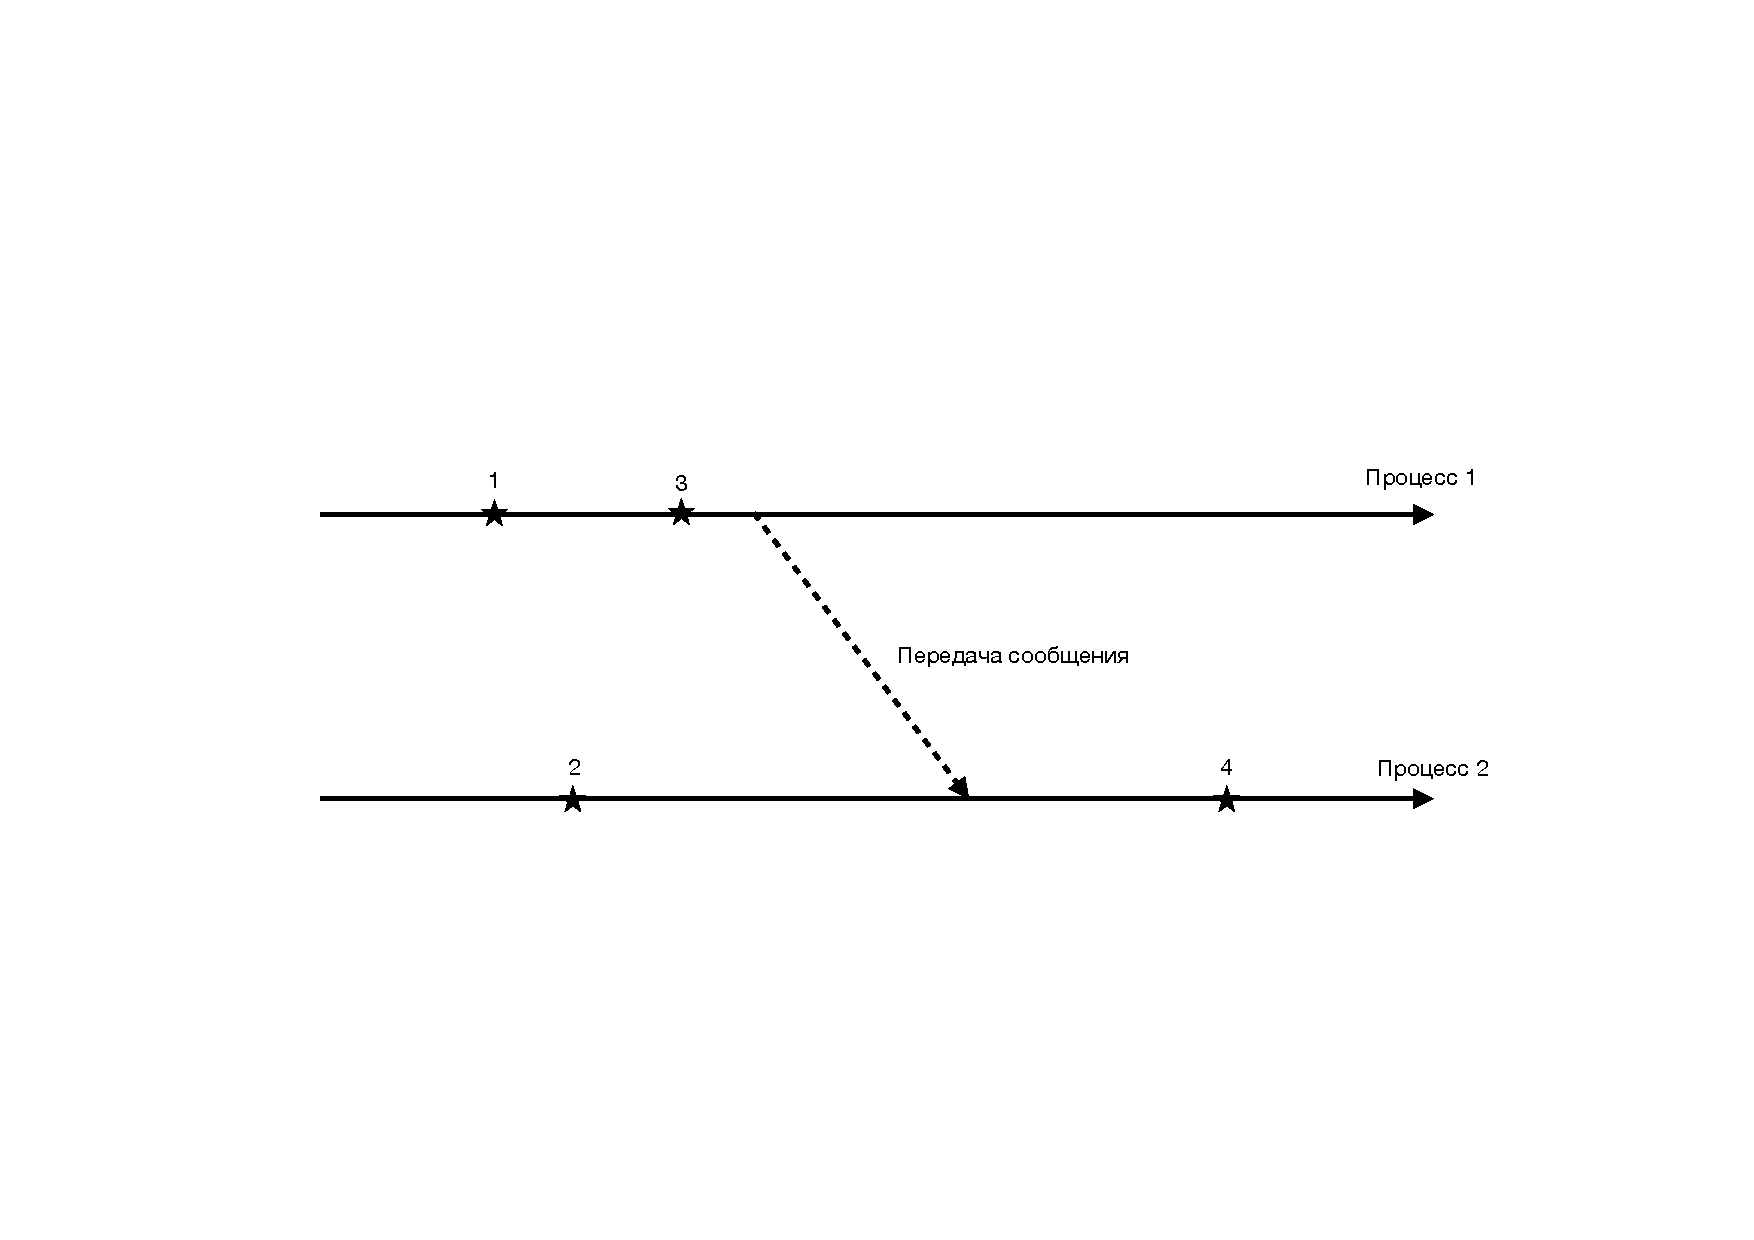
\includegraphics[scale=0.7]{15/masseg_time.pdf}

Так, на картинке, процесс 2 знает порядок событий в процессе 1 до передачи сообщения (события 1 и 3) и знает что они все были до события 4, но сравнить время событий 1 или 3 с временем событием 2 нельзя.
 
\textit{Более подробно этот пункт разобран в билете \ref{b20}.}
 
\item  Синхронные и асинхронные системы.

\hspace{12px}В \textbf{синхронной системе} предполагается, что каждое сообщение будет доставлено в течение некоторого заданного времени (если пакет не был доставлен за какое-то время, то он никогда не будет доставлен), а также известно время ответа любого узла (время выполнения операций).
Это позволяет пользователям моделировать протокол с фиксированной верхней границей, т.е. со значением максимального времени, требуемого на доставку сообщения принимающей стороне.

\hspace{12px}В \textbf{асинхронной системе} предполагается, что сеть может произвольно задерживать сообщения на любой период времени, дублировать или менять их порядок. Другими словами, фиксированная верхняя граница времени, необходимого на отправку и получение сообщения, отсутствует.

\hspace{12px} Асинхронная система менее удобная, но более распространённая в реальных распределённых системах, так как обычно компьютеры могут выходить из строя или уходить в автономный режим, а сообщения могут удаляться, дублироваться, задерживаться или поступать в произвольном порядке из-за проблем сети.
\end{itemize} 
\textbf{\noindent 2. Модели ошибок}

Отказ какого-то процесса может быть двух типов:
\begin{itemize}
\setlength\itemsep{0.0001em}
\item \textbf{Наблюдаемый отказ}  -  другие участники могут узнать, что он погиб.
\item \textbf{Ненаблюдаемый отказ}  - другие участники не могут узнать, что он погиб. Такие отказы более распространённые, поэтому, когда в алгоритме нужно найти гарантированно "живой" процесс, его часто ищут на основе таймеров, то есть если какой-то процесс не отвечает, то он начинает подозреваться в отказе.
\end{itemize}

\noindent Также ошибки могут быть следующих типов:

\textbf{Потеря} (в канале) - сообщение отправлено, но не дошло. 

\textbf{Пропуск отправки} (в процессе) - процесс не отправляет сообщения.

\textbf{Пропуск приема} (в процессе) - процесс не получает сообщения.

\textbf{Произвольное или византийское поведение} (и в канале, и в процессе) - поведение, не предписанное протоколом, возникшее из-за ошибок или же злоумышленно.\\
\\
\textbf{\noindent 3. Модели безопасности}

Политика информационной безопасности - документ на естественном языке.

Модель информационной безопасности - формализация этой политики, то есть выражение утверждений, написанных на русском языке, в терминах какого-то формального языка, а также реализация этой модели в распределённой системе. \\

В модели безопасности должны быть определенны:
\begin{itemize}
\item Описание информационной системы
\item Структурно-функциональные характеристики
\item Описание угроз безопасности
\item Модель нарушителя
\item Возможные уязвимости
\item Способы реализации угроз
\item Последствия от нарушения свойств безопасности информации.
\end{itemize}




